		\documentclass[a4paper,11pt]{report}


\usepackage[utf8]{inputenc}
\usepackage[T1]{fontenc}
\usepackage{lmodern}
\usepackage[norsk]{babel}
\usepackage{parskip}
\usepackage{graphicx}
\usepackage{titlepic}
\usepackage{a4wide}
\usepackage{color}
\usepackage{hyperref}
\usepackage{listings}
\lstdefinestyle{java1}{
  language=Java,
  basicstyle={\ttfamily\footnotesize},
  numberstyle={\ttfamily\footnotesize},
  keywordstyle={\ttfamily\footnotesize\color[rgb]{0,0,1}},
  commentstyle={\ttfamily\footnotesize\color[rgb]{0.133,0.545,0.133}},
  stringstyle={\ttfamily\footnotesize\color[rgb]{0.627,0.126,0.941}},
  breaklines=true,
  columns=fixed,
  extendedchars=true,
  numbers=left,
  numbersep=3pt,
  showspaces=false,
  showstringspaces=false,
  stepnumber=1,
  tabsize=2
}
\lstset{style=java1}
\renewcommand\lstlistingname{Eksempel}
\renewcommand\lstlistlistingname{Eksempler}

\usepackage{fancyhdr}
\setlength{\headheight}{15.2pt}
\pagestyle{fancy}
\fancypagestyle{plain}{ %
  \fancyhf{} % remove everything
  \renewcommand{\headrulewidth}{0pt} % remove lines as well
  \renewcommand{\footrulewidth}{0pt}
}

%Her kommer opsett av info for pdf filen
%\pdfinfo{%
%  /Title    (Rapport prosjektoppgave i programutvikling)
%  /Author   ()
%  /Creator  ()
%  /Producer ()
%  /Subject  ()
%  /Keywords ()
%}



\begin{document}
\begin{titlepage}
%\begin{center}
 



\title{Servicios De Vivienda}

\titlepic{
\includegraphics[width=40mm]{./img/fremside/logo.jpg}}

\author{Espen Zaal\\Lukas Larsed\\Petter Knagenhjelm Lysne}
\date{\today}



%\end{center}
\end{titlepage}

\maketitle
\begin{abstract}
Her kommer et sammendrag av rapporten. Skal normalt være ca en side. 
\end{abstract}
\tableofcontents
\lstlistoflistings
\listoffigures

\chapter{Bruksanvisning}

Stortingets Tibetkomité består av enkeltrepresentanter med et spesielt sterkt 
engasjement for Tibet. Etter stortingsvalget høsten 2013 tok Venstres Ketil 
Kjenseth på seg en koordinerende rolle, og sendte i januar ut en mail til alle 
stortingsrepresentanter om hvem som kunne tenke seg å bidra.
Til tross for at Høyre åpner sitt landsmøte på Gardermoen fredag formiddag har 
fem stortingsrepresentanter fra regjeringspartiet funnet plass i programmet til 
å møte tibetaneren: Michael Tetzschner, Heidi Nordby Lunde, Erik Skutle, Anders 
B. Werp og Peter Chr. Frølich. Også Unge Høyre-leder Paul Joakim Sandøy er med 
og tar imot Dalai Lama.

\section{Kode}
Her kommer litt javakode for å teste ut hvorda det kommer til å se ut.

\begin{lstlisting}[title=Eksempelkode, caption=Koden teller til 1000, label=brakode]
class KnappeLytter implements ActionListener {

        @Override
        public void actionPerformed(ActionEvent e) {
            if (e.getSource().equals(vindu.getLagreButton())) {
                if(erNyregistrering){
                    registrerNyLeietaker();
                }
            } else if (e.getSource().equals(vindu.getAvbrytButton())) {
                vindu.dispose();
            }
        }

    }
\end{lstlisting}


\section{Kode fra fil}
Slik kan man legge inn kode direkte fra en java fil

\lstinputlisting[title=Tellerklasse, caption=Koden her gir NullPointerException, label=kodelabel]{./kode/bruksanvisning/1.java}



\section{Liste}
Her kommer eksepel på en liste\footnote{Her legger man til en fotnot hvis man ønsker å kommentere noe.}
\begin{itemize}
 \item Epple
 \item Pære
 \item Frosker
 \item Banan
\end{itemize}



\section{Figurer}
\subsection{Eksempel 2}
\begin{figure}[ht]
 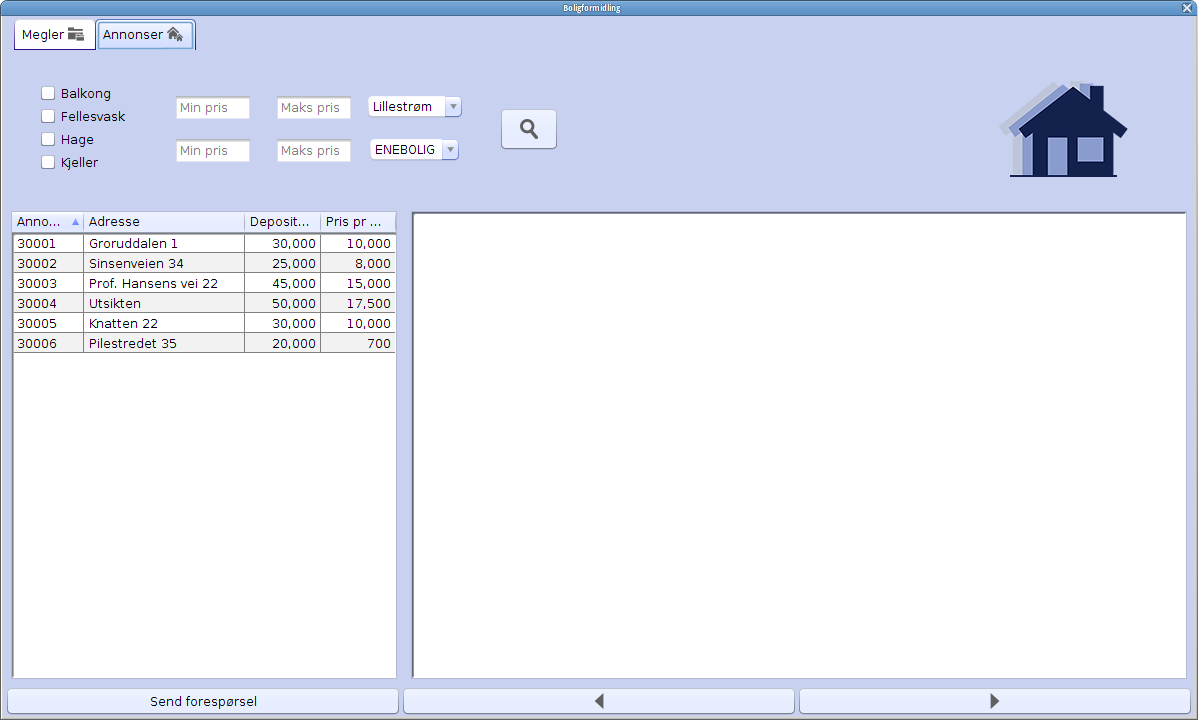
\includegraphics[width=\textwidth,height=\textheight,keepaspectratio]{./img/bruksanvisning/1.png}
 \caption{Dette er et eksempelbilde. Bilde blir automatisk numerert og lagt til i registeret.}
 %Her kommer en kabel for kryssreferering i teksten til figuren
 \label{fig:hovedvindu}
\end{figure}



\end{document}
